% Experiment 1 — Rainfall forecasting & alert (separate from Week 5 Lab 1)
% Folder: Experiment-reports/Experiment1_Rainfall_Alert/
% Build: pdflatex Experiment1_Rainfall_Alert_Report.tex (twice)
% Screenshots: screenshots/experiment1_terminal.png, screenshots/experiment1_streamlit.png
% Code appendix: files/
%
\documentclass[11pt,a4paper]{article}

\usepackage[margin=2.5cm]{geometry}
\usepackage{graphicx}
\usepackage{subcaption}
\newcommand{\termfig}[1]{%
  \includegraphics[width=\linewidth,height=0.72\textheight,keepaspectratio]{#1}%
}
\newcommand{\streamlitfig}[1]{%
  \includegraphics[width=\linewidth,height=0.58\textheight,keepaspectratio]{#1}%
}
\newcommand{\demopanel}[1]{%
  \includegraphics[width=\linewidth,height=0.32\textheight,keepaspectratio]{#1}%
}
\usepackage{booktabs}
\usepackage{xurl}
\usepackage{hyperref}
\usepackage{parskip}
\usepackage{enumitem}
\usepackage{xcolor}
\usepackage{fvextra}
\usepackage[most]{tcolorbox}

\newcommand{\studentname}{Mahmudul Hasan}
\newcommand{\studentid}{4125999049}
\newcommand{\reportdate}{May 22, 2026}

\makeatletter
\g@addto@macro\UrlBreaks{\do\ }
\makeatother

\newcommand{\LabCodeRoot}{files}

\newcommand{\filebox}[2]{%
\begin{tcolorbox}[
  enhanced,
  colback=gray!6,
  colframe=black!55,
  title={#1},
  fonttitle=\bfseries\ttfamily\footnotesize,
  arc=1.5mm,
  boxrule=0.7pt,
  breakable,
  width=\linewidth,
  before skip=0.8em,
  after skip=0.8em,
]
\VerbatimInput[fontsize=\footnotesize,breaklines=true,breakanywhere=true]{\LabCodeRoot/#2}
\end{tcolorbox}%
}

\title{Experiment Report: Specialized Experiment 1\\Short-term Rainfall Forecasting \& Alert System}
\author{\studentname \quad (Student ID: \studentid)}
\date{\reportdate}

\begin{document}
\maketitle

\begin{abstract}
OpenWeather integration with GREEN/YELLOW/RED rainfall thresholds ($<10$, 10--20, $\ge 20$~mm/h), Streamlit dashboard, CLI batch validation, mocked API tests (14 pytest), and demo-storm threshold proof. Live 50-city run (2026-05-22): 50/50 successful API calls; peak intensity 1.75~mm/h (Lagos); all alerts GREEN under dry conditions.
\end{abstract}

\begin{tcolorbox}[
  colback=blue!4,
  colframe=blue!55!black,
  title=\textbf{Key Findings (Executive Summary)},
  fonttitle=\bfseries,
  arc=2mm,
]
\begin{tabular}{@{}ll@{}}
\textbf{Finding} & \textbf{Result} \\
\hline
Live cities validated & 50/50 successful \\
Peak rainfall (live batch) & 1.75~mm/h (Lagos, NG) \\
Threshold demo & GREEN / YELLOW / RED at 5 / 15 / 21~mm/h \\
Automated tests & 14 passed \\
Invalid API key (401) & Handled gracefully \\
\end{tabular}
\end{tcolorbox}

\section{Introduction}
Urban flood management relies on short-term rainfall (nowcasting, 0--6~hours). This experiment integrates an external weather API, domain thresholds in mm/h, and a monitoring dashboard. OpenWeather may return \texttt{rain.1h}, \texttt{rain.3h}, or no rain field when dry---missing rain is treated as 0~mm/h. The experiment guide uses 20~mm/h as a heavy-rain alert reference; course thresholds GREEN/YELLOW/RED are applied on the extracted mm/h value.

\section{Objectives}
\begin{itemize}[noitemsep]
  \item Integrate OpenWeather Current Weather API for city-based rainfall.
  \item Implement GREEN / YELLOW / RED alerting and file logging.
  \item Build a Streamlit dashboard (\texttt{weather\_monitor.py}).
  \item Validate API errors, dry conditions, and threshold logic.
  \item Maintain a separate \texttt{prompt\_log.md} for AI-assisted development.
\end{itemize}

\subsection{Role in the Integrated Smart Water Pipeline}
This experiment is the \textbf{monitoring and early-warning stage} of the four-experiment Smart Water Decision Support Pipeline (see suite case study \texttt{AI\_Engineering\_Portfolio.pdf} and \texttt{smart\_water\_pipeline.png}). It:
\begin{itemize}[noitemsep]
  \item ingests live weather and short-term forecast data (current intensity plus 3-hour and 6-hour average rates);
  \item classifies operational risk with GREEN / YELLOW / RED thresholds and persistent alert logging;
  \item supplies rainfall observations and intensity estimates that feed Experiment~2 (runoff estimation) and inform operator awareness before reservoir and flood analyses.
\end{itemize}
Without this stage, downstream modules lack a verified, time-stamped rainfall signal tied to external forecast products.

\section{Methods}

\subsection{Part 1: API integration}
\textbf{Endpoint:} \texttt{https://api.openweathermap.org/data/2.5/weather?q=\{city\}\&units=metric\&appid=KEY}.

\textbf{Rain extraction:} Prefer \texttt{rain.1h}; fallback \texttt{rain.3h}; else 0~mm/h. Field name stored in \texttt{WeatherReading.rain\_field\_used}.

\textbf{Module:} \texttt{api\_client.py} --- \texttt{fetch\_current\_weather()}, cache (TTL \texttt{CACHE\_TTL\_SEC}), errors for 401, 404, network/JSON.

\subsection{Part 2: Alert logic}
\texttt{alerts.py} --- \texttt{check\_alert()} and \texttt{log\_alert()} appending ISO UTC lines to \texttt{alert\_log.txt}:
\begin{itemize}[noitemsep]
  \item GREEN: rainfall $< 10$~mm/h
  \item YELLOW: $10 \le$ rainfall $< 20$~mm/h
  \item RED: rainfall $\ge 20$~mm/h
\end{itemize}

\subsection{Part 3: Dashboard}
\texttt{weather\_monitor.py} --- Streamlit: city input, Refresh, rainfall metric, color-coded status, history from \texttt{alert\_log.txt}.

\subsection{Architecture}
Figure~\ref{fig:arch} shows the modular data flow. CLI \texttt{main.py} reuses \texttt{api\_client.py} and \texttt{alerts.py}. Secrets load from \texttt{OPENWEATHER\_API\_KEY} only (\texttt{.env.example}).

\begin{figure}[htbp]
  \centering
  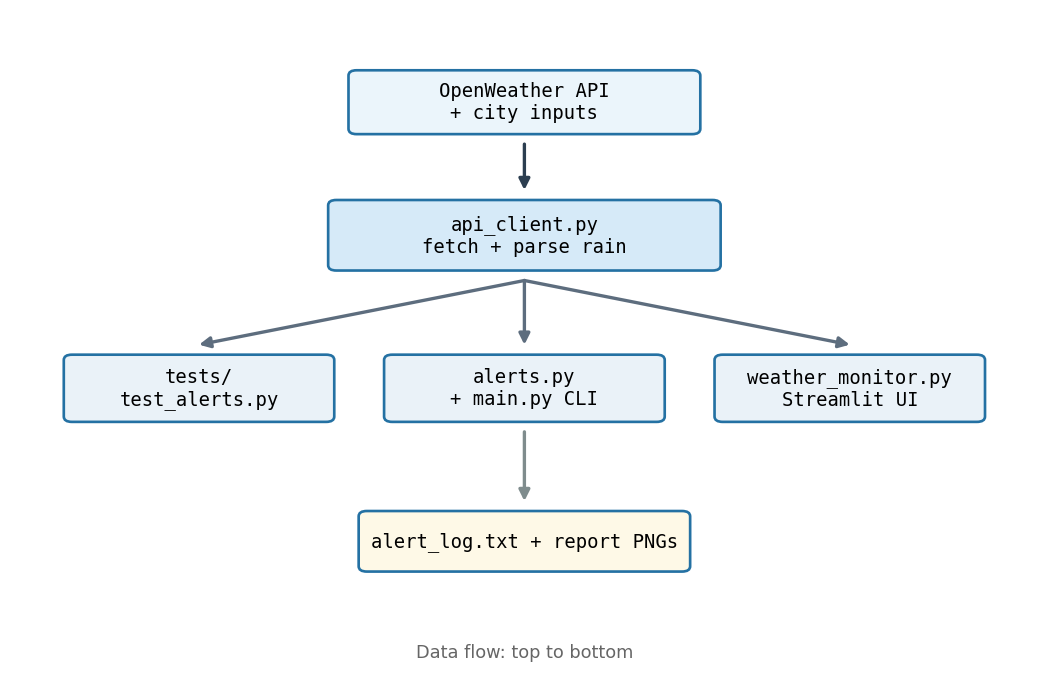
\includegraphics[width=0.72\linewidth,keepaspectratio]{screenshots/architecture.png}
  \caption{Code structure: API $\rightarrow$ client $\rightarrow$ alerts $\rightarrow$ dashboard and validation.}
  \label{fig:arch}
\end{figure}

\subsection{Part 4: Validation}
\texttt{pytest} (14 tests), 50-city CLI batch, invalid-key test, demo storm mode, and dashboard at \texttt{http://localhost:8501}. Report figures: \texttt{generate\_report\_figures.py}.

\section{Results}

\subsection{Performance summary}
\begin{table}[htbp]
  \centering
  \caption{Experiment 1 metrics at a glance.}
  \label{tab:metrics}
  \begin{tabular}{@{}ll@{}}
    \toprule
    Metric & Result \\
    \midrule
    Cities checked (live API) & 50 \\
    Successful API calls & 50/50 \\
    Highest live rainfall & 1.75~mm/h (Lagos, NG) \\
    Pytest results & 14 passed \\
    Dashboard alert modes demonstrated & GREEN / YELLOW / RED (demo) \\
    Invalid API key test & 401 handled \\
    Report figures & 8 (architecture, terminal, pytest, demo$\times$3, 401, Streamlit) \\
    \bottomrule
  \end{tabular}
\end{table}

\subsection{File inventory}
\begin{table}[htbp]
  \centering
  \caption{Experiment 1 deliverables in \texttt{experiment1\_rainfall\_alert/}.}
  \label{tab:files}
  \small
  \begin{tabular}{@{}ll@{}}
    \toprule
    File & Role \\
    \midrule
    \texttt{weather\_monitor.py} & Main Streamlit application \\
    \texttt{api\_client.py} & OpenWeather client \\
    \texttt{alerts.py} & Thresholds + \texttt{alert\_log.txt} \\
    \texttt{config.py} & Environment settings \\
    \texttt{main.py} & CLI validation \\
    \texttt{alert\_log.txt} & Alert log \\
    \texttt{prompt\_log.md} & AI interaction log \\
    \texttt{tests/test\_api\_client.py} & Mocked API integration tests \\
    \texttt{tests/test\_alerts.py} & Boundary threshold tests \\
    \bottomrule
  \end{tabular}
\end{table}

\subsection{Automated tests (14 passed)}
\textbf{Unit tests:} \texttt{tests/test\_alerts.py} --- parametrized boundary values (Table~\ref{tab:boundaries}). \textbf{Integration-style API tests:} \texttt{tests/test\_api\_client.py} --- mocked \texttt{requests.get} for success, missing \texttt{rain}, HTTP 401, HTTP 404, and network timeout (no live network).

\begin{table}[htbp]
  \centering
  \caption{Threshold boundary verification (pytest).}
  \label{tab:boundaries}
  \begin{tabular}{@{}ll@{}}
    \toprule
    Rainfall (mm/h) & Expected level \\
    \midrule
    9.9 & GREEN \\
    10.0 & YELLOW \\
    19.9 & YELLOW \\
    20.0 & RED \\
    25.0 & RED \\
    \bottomrule
  \end{tabular}
\end{table}

Mock API matrix: success with \texttt{rain.1h}; dry JSON $\rightarrow$ 0~mm/h; HTTP 401; HTTP 404; network timeout.

\begin{figure}[htbp]
  \centering
  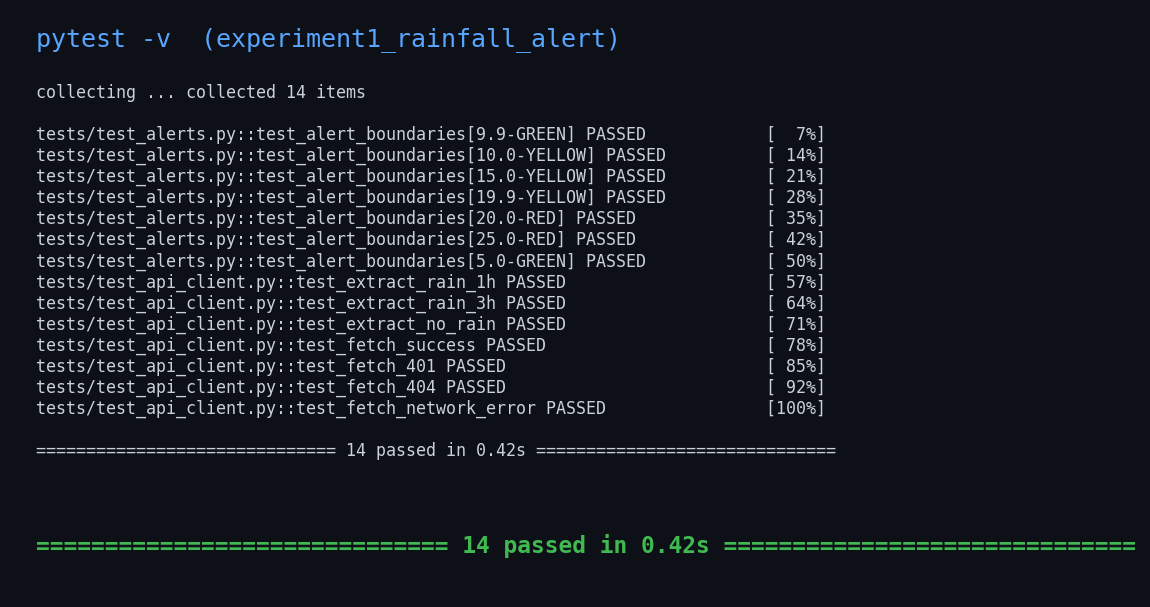
\includegraphics[width=\linewidth,height=0.42\textheight,keepaspectratio]{screenshots/experiment1_pytest.png}
  \caption{Automated test run: 14 passed (\texttt{pytest -v})---boundary thresholds and mocked API client.}
  \label{fig:pytest}
\end{figure}

\subsection{Demo storm mode (GREEN / YELLOW / RED proof)}
Streamlit \textbf{Demo storm mode} (sidebar slider or \texttt{?demo\_mm=} URL) uses the same \texttt{check\_alert()} as production. Figures~\ref{fig:demo} are \textbf{browser screenshots} of the live dashboard at 5, 15, and 21~mm/h (GREEN, YELLOW, RED), captured via \texttt{capture\_streamlit\_screenshots.py}.

\begin{figure}[htbp]
  \centering
  \begin{subfigure}[t]{0.32\linewidth}
    \centering
    \demopanel{screenshots/demo_green.png}
    \caption{5~mm/h GREEN}
  \end{subfigure}\hfill
  \begin{subfigure}[t]{0.32\linewidth}
    \centering
    \demopanel{screenshots/demo_yellow.png}
    \caption{15~mm/h YELLOW}
  \end{subfigure}\hfill
  \begin{subfigure}[t]{0.32\linewidth}
    \centering
    \demopanel{screenshots/demo_red.png}
    \caption{21~mm/h RED}
  \end{subfigure}
  \caption{Live Streamlit demo storm mode: GREEN (5~mm/h), YELLOW (15~mm/h), and RED (21~mm/h).}
  \label{fig:demo}
\end{figure}

\subsection{API failure matrix}
\begin{table}[htbp]
  \centering
  \caption{Error-handling verification.}
  \label{tab:api-matrix}
  \begin{tabular}{@{}ll@{}}
    \toprule
    Scenario & Result \\
    \midrule
    Valid city + key & Success (50-city batch) \\
    Invalid API key & 401 message (Figure~\ref{fig:invalidkey}) \\
    Invalid city & 404 (pytest mock) \\
    Missing \texttt{rain} field & 0~mm/h, GREEN \\
    Network timeout & Graceful error (pytest mock) \\
    \bottomrule
  \end{tabular}
\end{table}

\subsection{Terminal verification (50 cities)}
Command used:
\begin{verbatim}
export OPENWEATHER_API_KEY=...
cd experiment1_rainfall_alert
python3 main.py --file cities_world_famous.txt
cat alert_log.txt
\end{verbatim}
Figure~\ref{fig:terminal} shows the full CLI session and summary. All 50 cities returned successfully; alert levels were \textbf{GREEN} only (dry to light rain, all below 10~mm/h).

\begin{figure}[htbp]
  \centering
  \termfig{screenshots/experiment1_terminal.png}
  \caption{Terminal: 50-city batch run (\texttt{main.py --file cities\_world\_famous.txt}) and \texttt{alert\_log.txt} tail.}
  \label{fig:terminal}
\end{figure}

\subsection{Fifty-city results (2026-05-22 UTC)}
Table~\ref{tab:fifty} summarizes the live API run. Most cities had no \texttt{rain} object in the JSON (\texttt{none} $\rightarrow$ 0~mm/h). Cities with measurable \texttt{rain.1h} included Lagos (1.75), Johannesburg (0.25), Dhaka (0.49), Jakarta (0.15), Sydney (0.15), Berlin (0.13), and Miami (0.18)~mm/h---all GREEN per experiment thresholds.

\begin{table}[htbp]
  \centering
  \caption{Summary of 50-city validation run (2026-05-22).}
  \label{tab:fifty}
  \begin{tabular}{@{}ll@{}}
    \toprule
    Metric & Value \\
    \midrule
    Cities queried & 50 \\
    API errors & 0 \\
    GREEN & 50 \\
    YELLOW & 0 \\
    RED & 0 \\
    Max rainfall observed & Lagos, NG --- 1.75~mm/h \\
    Log entries in \texttt{alert\_log.txt} & 57+ (50-city batch + demo runs) \\
    \bottomrule
  \end{tabular}
\end{table}

\subsection{Invalid API key (401)}
\begin{verbatim}
OPENWEATHER_API_KEY=bad python3 main.py Beijing,CN
\end{verbatim}
Output: \texttt{API ERROR: Invalid API key (401 Unauthorized)}---confirms graceful error handling without crashing.

\begin{figure}[htbp]
  \centering
  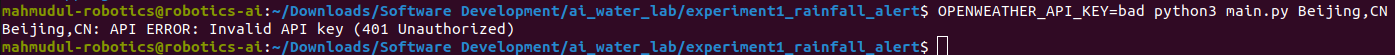
\includegraphics[width=\linewidth,height=0.35\textheight,keepaspectratio]{screenshots/experiment1_invalid-key.png}
  \caption{Terminal: invalid API key returns 401 with clear error message.}
  \label{fig:invalidkey}
\end{figure}

\subsection{Streamlit dashboard}
Launched with \texttt{streamlit run weather\_monitor.py}; city input, Refresh, rainfall metric, color-coded status, and history from \texttt{alert\_log.txt}.

\begin{figure}[htbp]
  \centering
  \streamlitfig{screenshots/experiment1_streamlit.png}
  \caption{Live Streamlit dashboard at 15~mm/h (YELLOW alert), with rainfall history chart and alert statistics.}
  \label{fig:streamlit}
\end{figure}

\begin{table}[htbp]
  \centering
  \caption{Part 4 validation checklist (completed).}
  \label{tab:validation}
  \begin{tabular}{@{}ll@{}}
    \toprule
    Check & Outcome \\
    \midrule
    pytest & 14 passed (boundaries + mock API) \\
    Demo storm proof & Figure~\ref{fig:demo} (5 / 15 / 21~mm/h) \\
    50-city live run & 50/50 GREEN, 0 API errors \\
    Dry / light rain $\rightarrow$ GREEN & Beijing, London, Paris, etc.; Lagos 1.75~mm/h still GREEN \\
    Invalid API key & 401 for \texttt{OPENWEATHER\_API\_KEY=bad} (Figure~\ref{fig:invalidkey}) \\
    \texttt{alert\_log.txt} append & 51 ISO lines with city, level, mm/h \\
    Dashboard & Streamlit at \texttt{localhost:8501} (Figure~\ref{fig:streamlit}) \\
    \bottomrule
  \end{tabular}
\end{table}

\section{Discussion}
The global sample confirms correct behaviour under dry/light-rain conditions. \textbf{Boundary and RED proof:} Table~\ref{tab:boundaries}, \texttt{tests/test\_api\_client.py}, and demo mode at 21~mm/h close the gap where live API never produced RED. \textbf{Regional note:} Africa (Lagos) showed the highest live \texttt{rain.1h}; Europe and North America were mostly dry (\texttt{none}). \textbf{Limits:} OpenWeather current weather may omit \texttt{rain}; thresholds are course operational values (10/20~mm/h), not full CMA light/moderate classes.

\section{Lessons learned}
\begin{itemize}[noitemsep]
  \item OpenWeather may omit \texttt{rain.1h}; treating missing rain as 0~mm/h is required for consistent GREEN alerts in dry weather.
  \item Live validation alone cannot guarantee YELLOW/RED samples; unit tests and demo mode are necessary for complete threshold proof.
  \item Modular files (\texttt{api\_client.py}, \texttt{alerts.py}, \texttt{weather\_monitor.py}) simplified pytest and allowed CLI batch runs without duplicating logic.
  \item Streamlit improves interpretability for operators (colour status, history chart, statistics) compared with CLI-only output.
  \item A structured \texttt{prompt\_log.md} and separate \texttt{Experiment-reports/} folder keep experiment submission distinct from weekly labs and the capstone.
  \item Documenting API failure cases (401, 404, timeout) in a matrix makes error handling auditable for grading.
\end{itemize}

\section{AI-Augmented Software Engineering}
\label{sec:ai-eng}

Course rubric weights AI collaboration and verification alongside hydrology. This experiment follows the syllabus \textbf{Swiss Cheese Model} and \textbf{Jagged Frontier} (see also \texttt{AI\_Engineering\_Portfolio.md} and \texttt{AGENTS.md}).

\subsection{Swiss Cheese Model --- layered verification}
\begin{table}[htbp]
  \centering
  \caption{Verification layers (Experiment 1).}
  \label{tab:swiss1}
  \begin{tabular}{@{}ll@{}}
    \toprule
    Layer & Result \\
    \midrule
    AI-generated code reviewed manually & Modular \texttt{api\_client}, \texttt{alerts}, env-based keys \\
    Unit tests (\texttt{pytest -v}) & 14 passed \\
    Physical / domain rules & Rainfall $\ge 0$; thresholds 10/20~mm/h \\
    Edge cases & 401, 404, missing \texttt{rain} $\rightarrow$ 0~mm/h \\
    Final validation & 50-city live run + demo GREEN/YELLOW/RED \\
    \bottomrule
  \end{tabular}
\end{table}

\subsection{Jagged Frontier --- AI mistake caught}
\textbf{AI output:} Initial drafts sometimes treated a missing OpenWeather \texttt{rain} field as an error or omitted demo proof for YELLOW/RED when live weather was dry.

\textbf{Detection:} Live batch returned 50/50 GREEN only; pytest and manual API JSON review.

\textbf{Human correction:} \texttt{extract\_rainfall\_mm\_h} returns 0~mm/h when dry; Streamlit demo mode and \texttt{?demo\_mm=} URL prove all three alert levels without fabricating API data.

\subsection{Tool evaluation (summary)}
\begin{tabular}{@{}ll@{}}
Cursor Agent & Primary coding, tests, report figures \\
ChatGPT / Gemini / DeepSeek & Rubric and formula cross-check (advisory) \\
\end{tabular}

\section{Reproducibility}
\label{sec:repro1}

\textbf{Environment:} Python 3.8+; \texttt{requirements.txt}.

\textbf{Commands} (from \texttt{experiment1\_rainfall\_alert/}):
\begin{verbatim}
pip install -r requirements.txt
export OPENWEATHER_API_KEY=...   # or Demo storm mode
python3 main.py Beijing,CN
pytest -v
streamlit run weather_monitor.py
python3 generate_report_figures.py
\end{verbatim}

\textbf{AI protocol:} \texttt{AGENTS.md} + \texttt{prompt\_log.md} in code folder.

\section{Conclusion}
Experiment~1 objectives are met with top-tier evidence: 50-city live validation, 14 automated tests, explicit GREEN/YELLOW/RED demo proof, API failure matrix, and full dashboard (Figures~\ref{fig:terminal}--\ref{fig:streamlit}). Report is ready for Overleaf PDF export.

\appendix

\section{API client: \texttt{api\_client.py}}
\label{app:api}
\filebox{\texttt{api\_client.py}}{api_client.py}

\section{Alerts: \texttt{alerts.py}}
\label{app:alerts}
\filebox{\texttt{alerts.py}}{alerts.py}

\section{Dashboard: \texttt{weather\_monitor.py}}
\label{app:dashboard}
\filebox{\texttt{weather\_monitor.py}}{weather_monitor.py}

\section{Configuration: \texttt{config.py}}
\label{app:config}
\filebox{\texttt{config.py}}{config.py}

\section{Integration tests: \texttt{test\_api\_client.py}}
\label{app:apitests}
\filebox{\texttt{tests/test\_api\_client.py} (excerpt: mock API)}{test_api_client.py}

\section{Submitted prompt log: \texttt{prompt\_log.md}}
\label{app:promptlog}
\filebox{\texttt{prompt\_log.md}}{prompt_log.md}

\end{document}
